\documentclass[../main.tex]{subfiles}
\newcommand\postcrit{P}
\newcommand\dist{\operatorname{dist}}
\newcommand\deriv[2]{{#1}'(#2)}
\begin{document}


\subsection{Siegel Discs and the Postcritical Closure}

In the previous sections, we've shown that every attracting periodic orbit attracts a critical point (Theorem \ref{8:thm:orbcrit}), and that every parabolic fixed point contains a critical point in each of its basins (Theorem \ref{10:lem:critical}). For an irrationally indifferent fixed point, there are again relations --- albeit less direct --- between the dynamics and the set of critical points.

\begin{dfn} The \emph{postcritical closure} $\postcrit$ of a map $f : \hat{\C} \to \hat{\C}$ is the topological closure of the strict forward orbits of the critical points of $f$:
\[
\postcrit = \postcrit(f) = \cl{\bigcup\limits_{n > 0} \iter{f}{n}(V)}
\]
in which $V = \{ z \in \hat{\C} \mid \deriv{f}{z} = 0\}$.
\end{dfn}

Equivalently, $\postcrit(f)$ is the smallest closed set that contains the critical values of $\iter{f}{n}$ for every $n > 0$. 

We have the following result:

\begin{thm}\label{11:thm:postcrit}
 $\postcrit(f)$ contains the attracting and superattracting periodic orbits of $f$, the indifferent periodic orbits of $f$ which lie in the Julia set, and the boundary of any domain on which $f$ is conjugate to a rotation. In particular, it contains every periodic orbit which is parabolic or Cremer, as well as the boundary of every period of Siegel discs.
\end{thm}

One proof of this theorem proceeds by endowing the complement $Q = \hat{\C}\setminus\postcrit(f)$ of the postcritical set with its Poincaré metric (this is possible so long as this complement is hyperbolic as a Riemann surface, which happens so long as $\postcrit(f)$ contains at least three points; in the case $\abs{\postcrit(f)} < 3$ it turns out that the map is always conjugate to $z \mapsto z^{\pm d}$ where $d \ge 2$ is the degree of $f$, and the dynamics of this exceptional case are well-understood.) It can then be demonstrated that the iterates $\iter{f}{k}$ expand the distances on $Q$, and \textit{strictly} expands distances at points in the Julia set whose forward orbits are disjoint from $Q$. These facts prohibit $Q$ from containing attracting fixed points, or indifferent fixed points in the Julia set. With some modifications, a similar argument can be applied to yield the conclusion for the boundaries of rotation domains. The details of the proof depend on more machinery than can be exposited within the length of this report in a satisfactory manner; we refer instead to the references (McMullen, 1994 and Milnor, 2006).

Propositions such as Theorem \ref{11:thm:postcrit} allow us to establish conclusions about the dynamics of the map by investigating the forward orbit of the critical set. (Nevertheless, we point out that there are cases where this is not very useful: for example, Rees (1942) demonstrates that there exist rational maps for which $\postcrit = \hat{\C}$.)

One might also attempt to further one's intuition of the dynamics of a map by computing these forward orbits and observing their behaviour. In the following we present a collection of computer-generated images, produced by the authors of this report, which are visually indicative of features of rational maps which have been discussed.

\begin{figure}[ht]
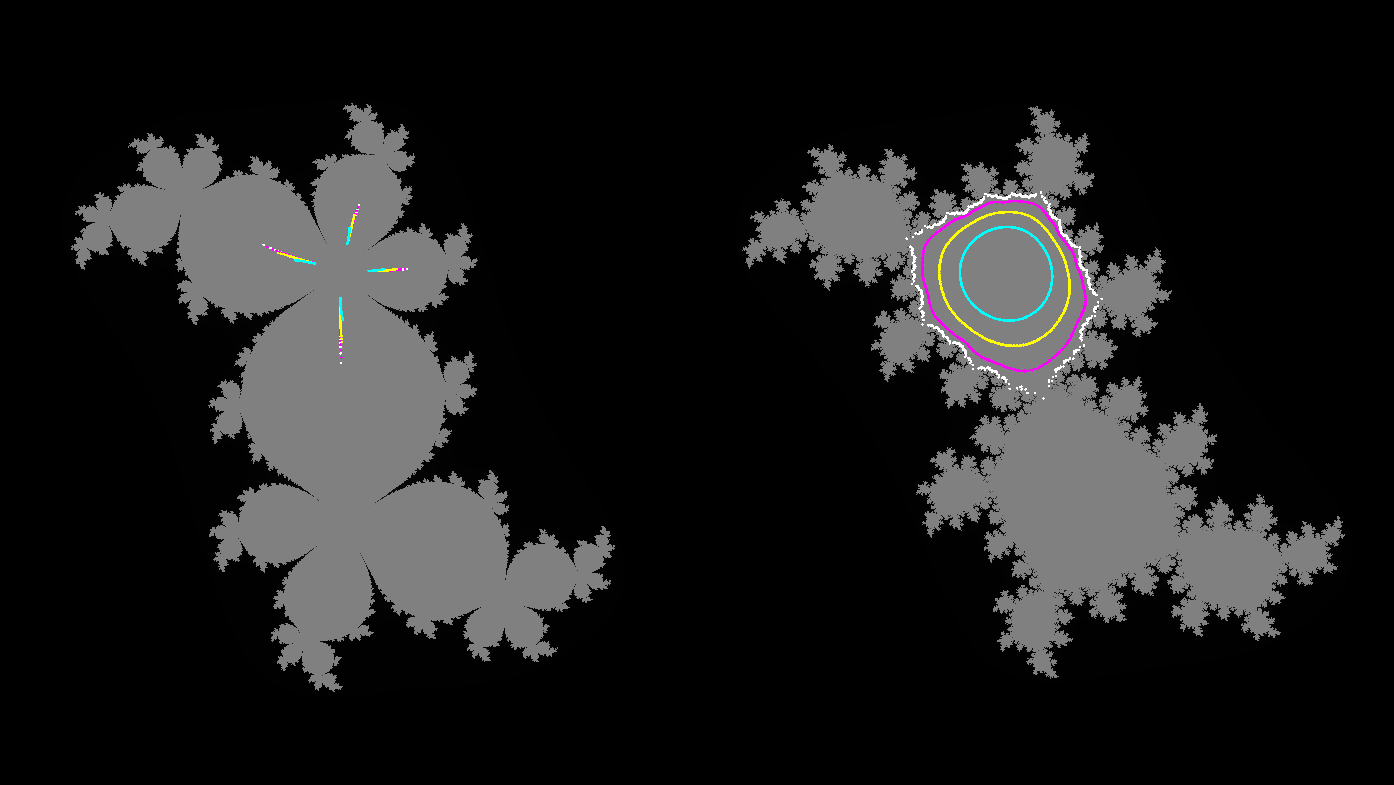
\includegraphics[width=\textwidth]{resources/ch-11/siegel/parabolic-and-siegel.png}
\caption{Filled Julia sets (grey) with the forward images of the critical point (white) and several nearby points (colours) plotted for a number of iterations. For $\xi \approx 0.2949$ (right), the forward orbit of the critical point delineates the boundary of a domain on which the dynamics are conjugated to a rotation, whereas for $\xi = 0.25$ (left) we observe convergence to a cycle of period 4.}
\end{figure}

\begin{figure}[ht]
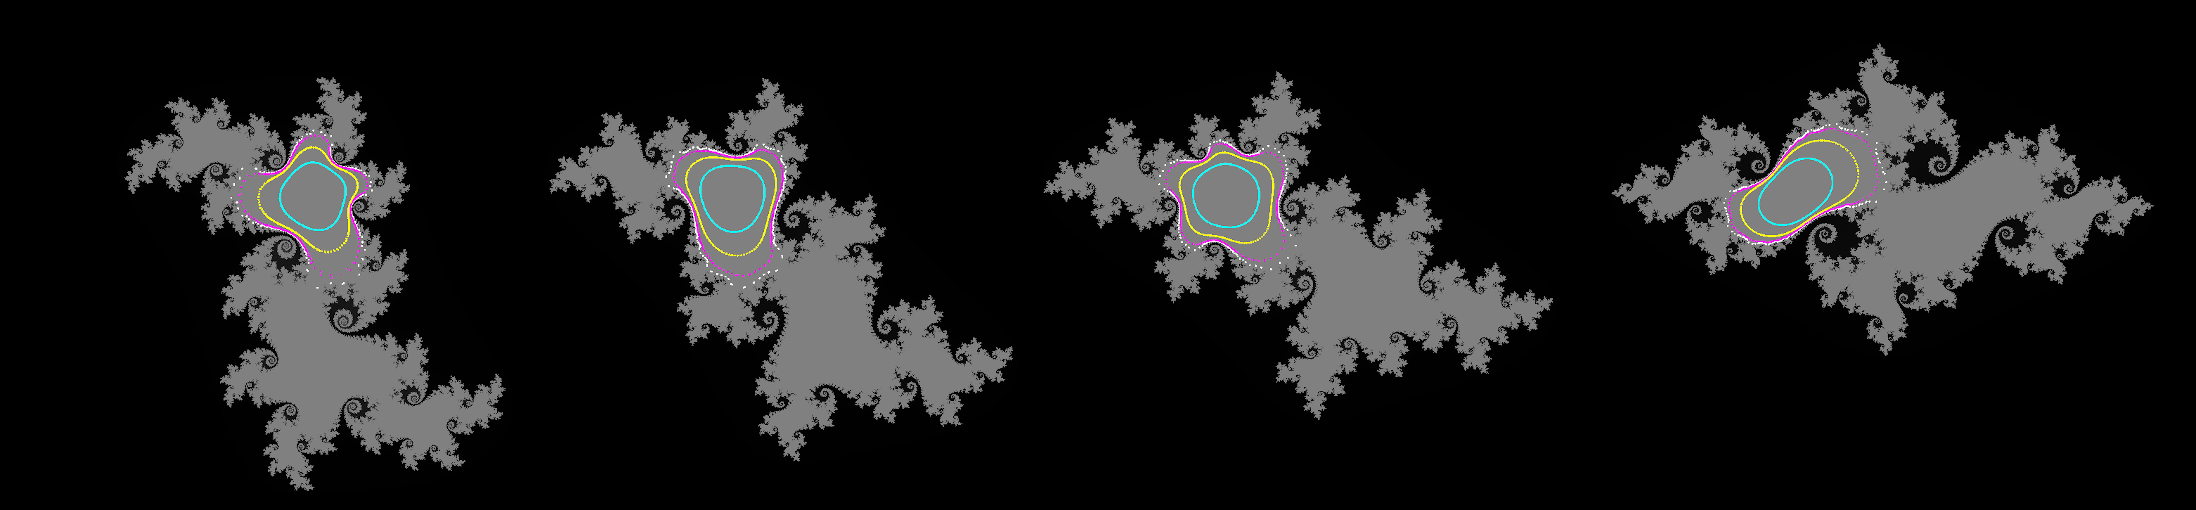
\includegraphics[width=\textwidth]{resources/ch-11/siegel/siegel-sequence.png}
\caption{Filled Julia sets and selected orbits for $\xi \approx 0.2475, 0.3408, 0.4023,$ and $0.4892$; the shape of the discs are suggestive of nearby rational numbers $(1/4, 1/3, 2/5, 1/2.)$}
\end{figure}

\end{document}